%%%%%%%%%%%%%%%%%%%%%%%%%%%%%%%%%%%%%%%%%%%%%%%%%%%%%%
\documentclass[11pt]{article}
%%%%%%%%%%%%%%%%%%%%%%%%%%%%%%%%%%%%%%%%%%%%%%%%%%%%%%

\usepackage{amsmath}
\usepackage{amsthm}
\usepackage{amssymb}
\usepackage{latexsym}
\usepackage{graphicx}
\usepackage{color}
\usepackage{verbatim}
\usepackage{float}
\usepackage{multicol}
\usepackage{xcolor}
\usepackage{listings}
\usepackage{tikz}
\usetikzlibrary{arrows.meta, positioning, calc}
\usetikzlibrary{decorations.pathmorphing}
\usepackage{tcolorbox}
\tcbuselibrary{breakable}

\newtcolorbox{solutionbox}{
  breakable,
  colback=blue!5!white,
  colframe=blue!50!black,
  title=Solution,
  sharp corners,
  boxrule=0.8pt
}

\newtcolorbox{hintbox}{
  breakable,
  colback=gray!10!white,
  colframe=gray!50!black,
  title=Hint,
  sharp corners,
  boxrule=0.5pt
}

% Unnumbered theorem
\newtheorem*{thm*}{Theorem}


\lstdefinelanguage{R}{
      keywords={if,else,while,for,in,next,break,function,TRUE,FALSE,NULL,Inf,NA,NaN,switch,repeat,return,require,library},
      keywordstyle=\color{blue}\bfseries,
      identifierstyle=\color{black},
      comment=[l]{\#},
      commentstyle=\color{gray}\ttfamily,
      string=[b]{"},
      stringstyle=\color{red}\ttfamily,
      morecomment=[l]{//},
      morestring=[b]{'},
      sensitive=true,
      morekeywords={print,summary,plot,lm,glm,data,frame,read.csv,write.csv,factor,levels,names,colnames,rownames,
      head,tail,str,dim,length,class,typeof,mode,is.na,is.null,is.finite,is.infinite,is.nan,as.numeric,as.character,
      as.factor,as.Date,as.POSIXct,as.matrix,as.data.frame,rbind,cbind,merge,subset,aggregate,tapply,apply,lapply,sapply,
      mapply,vapply,replicate,seq,rep,c,list,matrix,array,data.frame,table,hist,boxplot,barplot,pie,curve,lines,points,text,
      abline,legend,par,mtext,title,xlab,ylab,xlim,ylim,main,sub,col,pch,cex,lty,lwd,type,bg,fg,args,options,warnings,errors,
      message,stop,warning,error,try,tryCatch,withCallingHandlers,on.exit,debug,browser,trace,recover,options,getOption,setOption},
    }


\setlength{\textheight}{9in}
\setlength{\textwidth}{6in}
\addtolength{\topmargin}{-2cm}
\addtolength{\oddsidemargin}{-1cm}
\parindent=0in


\def\classnum{3810}
\def\classtitle{Probability}
\def\classtitleshort{Probability}
\def\classsec{001}
\def\classterm{Fall 2025}
\def\instructor{Robert Rostermundt}
%\def\hmwknum{\#2}


%%%%%%%%%%%%%%%%%%%%%%%%%%%%%%%%%%%%%%%%%%%%%%%%%%%%%%%%%
%%%%%%%%%%%%%%%%%%%%%%%%%  Colors  %%%%%%%%%%%%%%%%%%%%%%
%%%%%%%%%%%%%%%%%%%%%%%%%%%%%%%%%%%%%%%%%%%%%%%%%%%%%%%%%

\definecolor{Green}{rgb}{0,.5,0}
%use for definitions
\definecolor{Red}{rgb}{.8,.2,0}
%use for emphasis
\definecolor{Yellow}{rgb}{.6,.6,.1}
%use for part titles
\definecolor{Cyan}{rgb}{.2,.6,.7}
%use for comments
\definecolor{Purple}{rgb}{.4,0,1}
%use for examples
\definecolor{deepred}{rgb}{.53,.29,.24}
%use for important points
\definecolor{Black}{rgb}{0,0,0}
%use for washout
\definecolor{Grey}{rgb}{.45,.45,.45}
% use for theorems
\newcommand{\tred}[1]{\textcolor{Red}{#1}}
\newcommand{\tgreen}[1]{\textcolor{Green}{#1}}
\newcommand{\tcyan}[1]{\textcolor{Cyan}{#1}}
\newcommand{\tyellow}[1]{\textcolor{Yellow}{#1}}
\newcommand{\tpurple}[1]{\textcolor{Purple}{#1}}
\newcommand{\tblack}[1]{\textcolor{Black}{#1}}
\newcommand{\tgrey}[1]{\textcolor{Grey}{#1}}
\newcommand{\tdeepred}[1]{\textcolor{deepred}{#1}}
\newcommand{\ttt}[1]{\texttt{#1}}

%%%%%%%%%%%%%%%%%%%%%%%%%%%%%%%%%%%%%%%%%%%%%%%%%%%%%%%%%
%%%%%%%%%%%%%%%%%%%%%%%%%  Theorem Environments  %%%%%%%%
%%%%%%%%%%%%%%%%%%%%%%%%%%%%%%%%%%%%%%%%%%%%%%%%%%%%%%%%%

\theoremstyle{plain}
\newtheorem{thm}{Theorem}
\newtheorem{axiom}{Axiom}
\newtheorem{cor}{Corollary}
\newtheorem{lemma}{Lemma}
\newtheorem{prop}{Proposition}
\newtheorem{ques}{Question}
\theoremstyle{definition}
\newtheorem{defn}{Definition}
\theoremstyle{remark}
\newtheorem{remark}{Remark}
\theoremstyle{definition}
\newtheorem{ex}{Example}
\numberwithin{equation}{section}
\newtheorem{prob}{Problem}
\numberwithin{equation}{section}


%%%%%%%%%%%%%%%%%%%%%%%%%%%%%%%%%%%%%%%%%%%%%%%%%%%%%%%%%
%%%%%%%%%%%%%%%%%%%%%%%%%  Math    %%%%%%%%%%%%%%%%%%%%%%
%%%%%%%%%%%%%%%%%%%%%%%%%%%%%%%%%%%%%%%%%%%%%%%%%%%%%%%%%


\newcommand{\abs}[1]{\left\lvert{#1}\right\rvert}
\newcommand{\card}[1]{\lvert{#1}\rvert}
\newcommand{\union}{\cup}
\newcommand{\Union}{\bigcup}
\newcommand{\inter}{\cap}
\newcommand{\Inter}{\bigcap}
%\newcommand{\hint}[1]{\medskip\newline\emph{Hint: #1}}
%\newcommand{\note}[1]{\medskip\newline\emph{Note: #1}}
\newcommand{\points}[1]{[#1 points]}
\newcommand{\totalpoints}[1]{[#1 points total]}
\newcommand{\ds}{\displaystyle}
\newcommand{\ben}{\begin{enumerate}}
\newcommand{\een}{\end{enumerate}}
\newcommand{\bi}{\begin{itemize}}
\newcommand{\ei}{\end{itemize}}
\newcommand{\beq}{\begin{eqnarray*}}
\newcommand{\eeq}{\end{eqnarray*}}
\newcommand{\bieq}{\begin{IEEEeqnarray}{rCl}}
\newcommand{\bieqx}{\begin{IEEEeqnarray}{+rCl+x*}}
\newcommand{\eieq}{\end{IEEEeqnarray}}
\newcommand{\nn}{\nonumber}
%\renewcommand{\i}{\item}
\newcommand{\bpm}{\begin{pmatrix}}
\newcommand{\epm}{\end{pmatrix}}
\newcommand{\sol}{\indent{\bf\emph{Solution:}}}
\newcommand{\ssol}{\indent{\\[2mm]\bf\emph{Solution:}}\;}
\newcommand{\hint}{\indent{\bf\emph{Hint}:}\;}
\newcommand{\note}{\indent{\bf\emph{Note}:}\;}
\newcommand{\vsk}{\vskip 2mm}
%%%%%%%%%%%%%%%%%%%%%%%%% Calculus %%%%%%%%%%%%%%%%%%%%%%%%%%%%
\newcommand{\dd}[2]{\ds\frac{d}{d{#1}}\left[{#2}\right]}
\newcommand{\der}[2]{\ds\frac{d{#1}}{d{#2}}}
\newcommand{\lmt}[3]{\ds\lim_{{#1}\to{#2}}{#3}}
\renewcommand{\iint}[2]{\ds\int{#1}\,d{#2}}
\newcommand{\dint}[4]{\ds\int^{#4}_{#3}{#1}\,d{#2}}
\renewcommand{\Delta}{\triangle}
%%%%%%%%%%%%%%%%%%%%%%%%% Number Sets %%%%%%%%%%%%%%%%%%%%%%%%%%
\newcommand{\N}{\mathbb{N}}
\newcommand{\Z}{\mathbb{Z}}
\newcommand{\Q}{\mathbb{Q}}
\newcommand{\R}{\mathbb{R}}
\newcommand{\C}{\mathbb{C}}
\newcommand{\F}{\mathcal{F}}
\renewcommand{\P}{\mathbb{P}}
\newcommand{\E}{\mathcal{E}}
\renewcommand{\o}{\omega}
\renewcommand{\O}{\Omega}
%%%%%%%%%%%%%%%%%%%%%%%%% Vectors %%%%%%%%%%%%%%%%%%%%%%%%%%%%%
\newcommand{\x}{\bar{x}}
\renewcommand{\v}{\bar{v}}
\newcommand{\y}{\bar{y}}
\newcommand{\z}{\bar{z}}
\newcommand{\w}{\bar{w}}
\renewcommand{\u}{\bar{u}}
\renewcommand{\b}{\bar{b}}
\newcommand{\e}{\bar{e}}
\renewcommand{\a}{\vec{a}}
\renewcommand{\r}{\vec{r}}
\newcommand{\vv}{\vec{v}}
\newcommand{\vecPQ}[2]{\overrightarrow{#1}{#2}}
\newcommand{\vecV}[1]{\overrightarrow{#1}}
\newcommand{\la}{\langle}
\newcommand{\ra}{\rangle}
%%%%%%%%%%%%%%%%%%%%%%%%%%% Vector Spaces %%%%%%%%%%%%%%%%%%%%
\newcommand{\rn}{\ensuremath{\mathbb{R}^n}}
\renewcommand{\rm}{\ensuremath{\mathbb{R}^m}}
\newcommand{\re}{\mathbb{R}}
\newcommand{\Pn}{\mathbb{P}_n}
\newcommand{\B}{\mathcal{B}}
%%%%%%%%%%%%%%%%%%%%%%%%%%% Graphics %%%%%%%%%%%%%%%%%%%%%%%%
\newcommand{\cg}[2]{\begin{center}
\includegraphics[scale={#1}]{{#2}}
\end{center}}
\makeatletter
\def\imod#1{\allowbreak\mkern10mu({\operator@font mod}\,\,#1)}
\makeatother

%%%%%%%%%%%%%%%%%%%%%%%%%%%%%%%%%%%%%%%%%%%%%%%%%%%%%%%%%%%%%%%%%%%%%%%%%%%%%%%%%%%%%%%%%%%%%%
%%%%%%%%%%%%%%%%%%%%%%%%%%%%%% Defined Fonts %%%%%%%%%%%%%%%%%%%%%%%%%%%%%%%%%%%%%%%%%%%%%%%%%
%%%%%%%%%%%%%%%%%%%%%%%%%%%%%%%%%%%%%%%%%%%%%%%%%%%%%%%%%%%%%%%%%%%%%%%%%%%%%%%%%%%%%%%%%%%%%%

\font\minihelv=phvr at 6pt
\font\helv=phvr at 10pt
\font\medhelv=phvr at 16pt
\font\bighelv=phvr at 20pt
\font\hugehelv=phvr at 36pt
\font\mybigfont=phvr at 16pt
\font\mymediumfont=phvr at 14pt
\font\mediumhelv=phvr at 14pt
\font\mybfit=ptmbi at 12pt


%%%%%%%%%%%%%%%%%%%%%%%%%%%%%%%%%%%%%%%%%%%%%%%%%%%%%%%%%%%%%%%%%%%%%%%%%%%%%%%%%%%%%%%%%%%%%%%
%%%%%%%%%%%%%%%%%%%%%%%%%%%%%% Other Commands %%%%%%%%%%%%%%%%%%%%%%%%%%%%%%%%%%%%%%%%%%%%%%%%%
%%%%%%%%%%%%%%%%%%%%%%%%%%%%%%%%%%%%%%%%%%%%%%%%%%%%%%%%%%%%%%%%%%%%%%%%%%%%%%%%%%%%%%%%%%%%%%%
%\setlength\fboxrule{.5pt}
%\newcommand{\latexpicborder}[3]{
%\setlength\fboxsep{30pt}
%\begin{figure}[hb]
%\begin{center}
%\fbox{
%\input{#1}
%}
%\caption{#2}
%\label{#3}
%\end{center}
%\end{figure}
%\setlength\fboxsep{0pt}
%}
%
%\newcommand{\latexpic}[2]{
%\begin{figure}[hb]
%\begin{center}
%\input{#1}
%\vspace*{8mm}
%\caption{#2}
%\end{center}
%\end{figure}
%}

%\begin{minipage}[b]{0.6\linewidth}
%......
%\end{minipage}
%\hspace{0.5cm}
%\begin{minipage}[t]{0.4\linewidth}
%\centering
%\includegraphics[scale=.5]{m1401_ex3_g4.eps}
%\end{minipage}
%\end{figure}


%%%%%%%%%%%%%%%%%%%%%%%%%%%%%%%%%%%%%%%%%%%%%%%%%%%%%%%%%%%%%%%%%%%%%%%%%%%%%%%%%%%%%%%%%%%%%%
%%%%%%%%%%%%%%%%%%%%%%%%%%% IEEEeqnarray Notes %%%%%%%%%%%%%%%%%%%%%%%%%%%%%%%%%%%%%%%%%%%%%%%
%%%%%%%%%%%%%%%%%%%%%%%%%%%%%%%%%%%%%%%%%%%%%%%%%%%%%%%%%%%%%%%%%%%%%%%%%%%%%%%%%%%%%%%%%%%%%%


%Any number of columns can be specified with IEEEeqnarray: {c} will give only one
%column with all entries centered, or {rCll} would add a fourth, left-justified
%column to use for comments. Moreover, beside l, c, r, L, C, R for math mode
%entries there are also s, t, u for left, centered, and right text mode entries.
%Additional space can be added with . and / and ? in increasing order.
%
%
%\begin{proof}
%This is a proof that ends
%with an equation array:
%\begin{IEEEeqnarray*}{+rCl+x*}
%a & = & b + c \\
%& = & d + e. & \qedhere
%\end{IEEEeqnarray*}
%\end{proof}
%Note that the + in {+rCl+x*} denotes stretchable spaces, one on the left
%of the equations (which, if not specified, will be done automatically by
%IEEEeqnarray!) and one on the right of the equations. But now on the right,
%after the stretching column, we add an empty column x. This column will be
%only needed on the last line when we will put the \qedhere command there.
%Finally, we specify a *. This is a null-space that prevents IEEEeqnarray to
%add another unwanted +-space!


% The following environments enable custom numbering of theorems so that the numbers agree % with the numbering in the textbook being used. 
%
%  Usage examples:
%\begin{customthm}{2.2}\label{eight}
%Every theorem must be numbered by hand.
%\end{customthm}
%
%Here is a reference to theorem~\ref{eight}.
%
%\begin{customthm}{2.3}[Parenthetical comment]\label{nine}
%Statement
%\end{customthm}
%
%Here is a reference to theorem~\ref{nine}


\newtheorem{innercustomthm}{Theorem}
\newenvironment{customthm}[1]
  {\renewcommand\theinnercustomthm{#1}\innercustomthm}
  {\endinnercustomthm}
  
  \newtheorem{innercustomprop}{Proposition}
\newenvironment{customprop}[1]
  {\renewcommand\theinnercustomprop{#1}\innercustomprop}
  {\endinnercustomprop}
  
    \newtheorem{innercustomlem}{Lemma}
\newenvironment{customlem}[1]
  {\renewcommand\theinnercustomlem{#1}\innercustomlem}
  {\endinnercustomlem}
  
    \newtheorem{innercustomconj}{Conjecture}
\newenvironment{customconj}[1]
  {\renewcommand\theinnercustomconj{#1}\innercustomconj}
  {\endinnercustomconj}
  
    \newtheorem{innercustomclaim}{Claim}
\newenvironment{customclaim}[1]
  {\renewcommand\theinnercustomclaim{#1}\innercustomclaim}
  {\endinnercustomclaim}
  
    \newtheorem{innercustomcor}{Corollary}
\newenvironment{customcor}[1]
  {\renewcommand\theinnercustomcor{#1}\innercustomcor}
  {\endinnercustomcor}
  
    \newtheorem{innercustomdef}{Definition}
\newenvironment{customdef}[1]
  {\renewcommand\theinnercustomdef{#1}\innercustomdef}
  {\endinnercustomdef}
  
    \newtheorem{innercustomex}{Example}
\newenvironment{customex}[1]
  {\renewcommand\theinnercustomex{#1}\innercustomex}
  {\endinnercustomex}
  
    \newtheorem{innercustomass}{Assumption}
\newenvironment{customass}[1]
  {\renewcommand\theinnercustomass{#1}\innercustomass}
  {\endinnercustomass}
  
      \newtheorem{innercustomax}{Axiom}
\newenvironment{customax}[1]
  {\renewcommand\theinnercustomax{#1}\innercustomax}
  {\endinnercustomax}
  

\vfuzz2pt % Don't report over-full v-boxes if over-edge is small
\hfuzz2pt % Don't report over-full h-boxes if over-edge is small

\renewcommand{\ni}{\noindent}


%%%%%%%%%%%%%%%%%%%%%%%%%%%%%%%%%%%%%%%%%%%%%%%%%%%%%%
%%%%%%%%%%%%%%%%%%%%%%%%%%%%%%%%%%%%%%%%%%%%%%%%%%%%%%

\pagestyle{myheadings}

%%%%%%%%%%%%%%%%%%%%%%%%%%%%%%%%%%%%%%%%%%%%%%%%%%%%%%

%%%%%%%%%%%%%%%%%%%%%%%%%%%%%%%%%%%%%%%%%%%%%%%%%%%%%%
%%%%%%%%%%%%%%%%%%%%%%%%%   Document Body   %%%%%%%%%%
%%%%%%%%%%%%%%%%%%%%%%%%%%%%%%%%%%%%%%%%%%%%%%%%%%%%%%

%\def\classnum{3810}
%\def\classtitle{Probability}
%\def\classtitleshort{Probability}
%\def\classsec{001}
%\def\classterm{Fall 2025}
%\def\instructor{Robert Rostermundt}
\def\printsol{0}


	\title{\vspace{-1in}Math\classnum\;-\;\classtitle\\
	Section\;\classsec\;-\;\classterm\\
	Notes: General Random Variables}
	\author{University of Colorado Denver / College of Liberal Arts 	and Sciences}
	\date{Department of Mathematics - \instructor}

	\markright{Math\classnum\;-\;\classtitleshort, UCD, \classterm, \instructor}



%%%%%%%%%%%%%%%%%%%%%%%%%%%%%%%%%%%%%%%%%%%%%%%%%%%%%%
\begin{document}\maketitle\thispagestyle{empty}
%%%%%%%%%%%%%%%%%%%%%%%%%%%%%%%%%%%%%%%%%%%%%%%%%%%%%%


%%%%%%%%%%%%%%%%%%%%%%%%%%%%%%%%%%%%%%%%%%%%%%%%%%%%%%%%%%%%%%%%%%%%%%%%%%%%%%%%%%%%%%%%%%%%%%%%%%%%%%
\vspace*{2mm}
\hrule
\vskip 8mm


%%%%%%%%%%%%%%%%%%%%%%%%%%%%%%%%%%%%%%%%%%%%%%%%%%%%%%%%%%%%%%%%%%%%%%%%%
%%%%%%%%%%%%%%%%%%%%%%%%%%%%%%%%%%%%%%%%%%%%%%%%%%%%%%%%%%%%%%%%%%%%%%%%%


%%%%%%%%%%%%%%%%%%%%%%%%%%%%%%%%%%%%%%%%%%%%%%%%%%%%%%%%%%%%%%%%%%%%%%%%%%%%%%%%%%%%%%%%%%%%%%%%%%%%%%
\section*{Motivation:}
%%%%%%%%%%%%%%%%%%%%%%%%%%%%%%%%%%%%%%%%%%%%%%%%%%%%%%%%%%%%%%%%%%%%%%%%%%%%%%%%%%%%%%%%%%%%%%%%%%%%%%


\noindent In probability theory, a \emph{random variable} is a way of assigning a numerical value to each outcome in a probability space. This allows us to quantify uncertain events and compute probabilities, expected values, and other statistical measures.

\medskip

\textbf{Motivating example: Gambling with dice.} Suppose you roll two fair six-sided dice. Let the sample space be 
\[
\Omega = \{(i,j) : i,j = 1,2,3,4,5,6\}.
\] 
Instead of only asking about which pair of numbers appears, imagine a gambling game where you receive different monetary payouts depending on the dice roll:
\begin{itemize}
    \item If the sum of the dice is 7, you win \$10.
    \item If the sum is 2 or 12, you win \$5.
    \item Otherwise, you lose \$2.
\end{itemize}

Here, the \emph{random variable} \(X\) represents your winnings: 
\[
X: \Omega \to \mathbb{R}, \quad X(i,j) =
\begin{cases} 
10 & \text{if } i+j = 7,\\
5 & \text{if } i+j = 2 \text{ or } 12,\\
-2 & \text{otherwise}.
\end{cases}
\]

This example illustrates the general idea: a random variable maps each outcome \(\omega \in \Omega\) to a numerical value \(X(\omega)\). Once we have \(X\), we can compute probabilities of events such as ``winning money” (\(X>0\)), the expected payout, or other statistics of interest.  

\medskip

This perspective allows us to move beyond simple outcomes and reason about numerical quantities associated with complex events in any probability model.


%%%%%%%%%%%%%%%%%%%%%%%%%%%%%%%%%%%%%%%%%%%%%%%%%%%%%%%%%%%%%%%%%%%%%%%%%%%%%%%%%%%%%%%%%%%%%%%%%%%%%%
\section*{Random Variables:}
%%%%%%%%%%%%%%%%%%%%%%%%%%%%%%%%%%%%%%%%%%%%%%%%%%%%%%%%%%%%%%%%%%%%%%%%%%%%%%%%%%%%%%%%%%%%%%%%%%%%%%


\begin{defn}
Given a probability space $(\O,\F,\P)$, a {\bf\emph{random variable}} is an $\F$-measurable function $X:\O\to\R$.
\end{defn}

\ni {\bf\emph{Note}}: An $\F$-measureable function is a function so that for every Borel set $B\in 2^{\R}$, we must have the preimage $X^{-1}(B)\in\F$; i.e., 
\[X^{-1}(B)=\left\{\o\in\O:X(\o)=x\right\}\in\F.\]
If we let $\mathcal{C}_0$ be the set of all open intervals on the real line, we call the smallest $\sigma$-algebra containing 
$\mathcal{C}_0$, denoted $\mathcal{B}(\R)$, the Borel $\sigma$-algebra. A Borel set is an element of $\mathcal{B}(\R)$. The point is we need to be able to assign probabilities to the set $X^{-1}(\mathcal{B})$, and so all such preimages must be events.\\

\ni We want to assign probabilities to subsets of $Im(X)$. That is, we want to assign a {\bf\emph{probability law}}, denoted $\P_{X}$, to $X$. We do this in the following way: 
\[\P_{_X}:\mathcal{B}(\R)\to[0,1],\text{ where }\P_{_X}\big(B\big)\mapsto\P\big(X^{-1}(B)\big).\]
So the probability law for $X$ is the composition of $X^{-1}$ and the original probability measure $\P$. That is, 
\[\P_{_X}=\P\circ X^{-1}.\] 
See the diagram in Figure~\ref{fig:problaw} below.
\vskip 1cm

%%%%%%%%%%%%%%%%%%%%%%%%%%%%%%%%%%%%%%%%%%%%%%%%%%%%%%%%%%%%%%%%%%%%
% Randon Variable Diagram
%%%%%%%%%%%%%%%%%%%%%%%%%%%%%%%%%%%%%%%%%%%%%%%%%%%%%%%%%%%%%%%%%%%%

\begin{figure}[h!]
	\begin{center}
		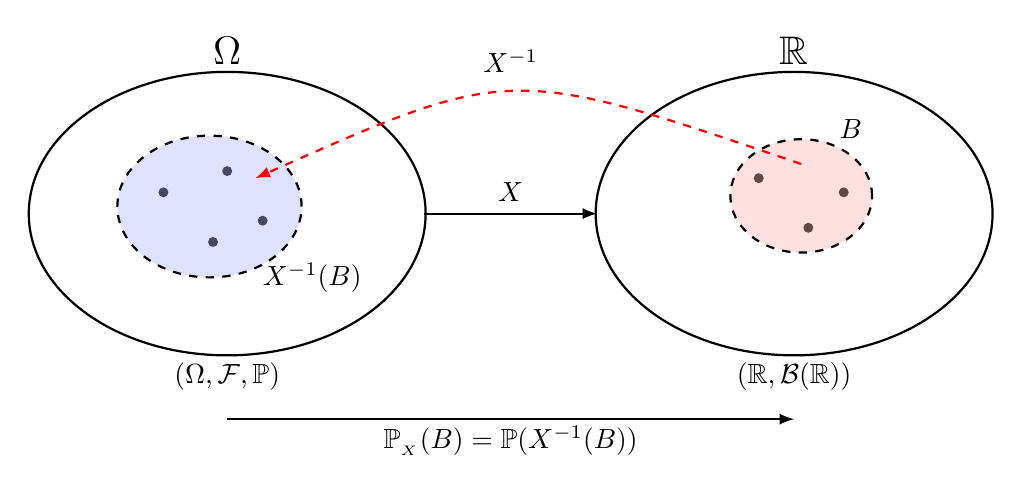
\begin{tikzpicture}[scale=0.9, >=latex]

% --- Sample space Omega ---
\draw[thick] (-4,0) ellipse (2.8 and 2.0);
\node at (-4,2.3) {\Large $\Omega$};
\node at (-4,-2.3) {$(\Omega,\mathcal F,\mathbb P)$};

% sample points in Omega 
\fill (-4.9,0.3) circle (2pt); % in X^{-1}(B)
\fill (-4,0.6) circle (2pt);
\fill (-4.2,-0.4) circle (2pt); % in X^{-1}(B)
\fill (-3.5,-0.1) circle (2pt);

% --- Subset in Omega: X^{-1}(B) ---
\draw[thick, dashed, fill=blue!30, fill opacity=0.4] (-4.25,0.1) ellipse (1.3 and 1.0);
\node at (-2.8,-0.9) {$X^{-1}(B)$};

% --- Real line / codomain ---
\draw[thick] (4,0) ellipse (2.8 and 2.0);
\node at (4,2.3) {\Large $\mathbb R$};
\node at (4,-2.3) {$(\mathbb R,\mathcal B(\mathbb R))$};

% image points in R 
\fill (3.5,0.5) circle (2pt); % in B
\fill (4.2,-0.2) circle (2pt);
\fill (4.7,0.3) circle (2pt); % in B

% --- Subset in R: B  ---
\draw[thick, dashed, fill=red!30, fill opacity=0.4] (4.1,0.25) ellipse (1.0 and 0.8);
\node at (4.8,1.2) {$B$};

% --- Arrow X (stays between the sets) ---
\draw[->, thick] (-1.22,0) -- (1.22,0);
\node at (0,0.3) {$X$};

% --- Dashed inverse image arrow ---
\draw[dashed, thick, red, ->] (4.1,0.7) .. controls (0,2.1) .. (-3.6,0.5);
\node at (0,2.15) {$X^{-1}$};

% --- Probability arrows ---
\draw[->, thick] (-4,-2.9) -- (4,-2.9);
\node at (0,-3.2) {$\mathbb P_{_X}(B)=\mathbb P(X^{-1}(B))$};

		\end{tikzpicture}
\caption{Probability Law For a Random Variable $X$.}
\label{fig:problaw}
	\end{center}
\end{figure}
\vskip 5mm

%%%%%%%%%%%%%%%%%%%%%%%%%%%%%%%%%%%%%%%%%%%%%%%%%%%%%%%%%%%%%%%%%%%%%%%%%%%%%%%%%%%%%%%%%%


A function called the distribution function of $X$ is one of the most important tools for working with random variables.
\vskip 5mm
\begin{defn}
Let $X$ be a random variable with a corresponding probability space $(\O,\F,\P)$. Then we define the {\bf\emph{distribution function}} $F_{_X}$ as
\[F_{_X}(x)=\P_{_X}\Big((-\infty,x]\Big)=\P\Big(\big\{\o\in\O:X(\o)\le x\big\}\Big).\]
\end{defn}

\ni {\bf\emph{Note}}: It can be shown that the distribution function $F_{X}$ completely determines the probability law $\P_{X}$; i.e., once we have defined the probability law for all sets $(-\infty,x]$, there is a unique way to extend this probability law to the Borel $\sigma$-algebra $\mathcal{B}(\R)$.\\

\ni There are a few distinguishing characteristics of a distribution which we list below. A proof follows at the end of the document.\\

\begin{thm}\label{thm:distribution}
Let $(\O,\F,\P)$ be a probability space and $X:\F\to\
R$ be a random variable with distribution function $F_{_X}$. Then the following properties hold.

	\begin{enumerate}
	
		\item $\ds\lim_{x\to-\infty}F_{_X}(x)=0$;
		\item $\ds\lim_{x\to\infty}F_{_X}(x)=1$;
		\item $F_{_X}$ is monotonically increasing everywhere; i.e., if $x\le y$, then $F_{_X}(x)\le F_{_X}(y)$.
		\item $F_{_X}$ is right-continuous; i.e., for all $x\in\R$ we have 
$\ds\lim_{\epsilon\to 0^+}F_{_X}(x+\epsilon)=F_{_X}(x)$. 
		
	\end{enumerate}
	
\end{thm}

\ni{\bf\emph{Note}}: Some distribution functions, such as for a continuous random variable, will also be left-continuous; i.e., and so continuous, but many random variables, such as discrete random variables will not be left-continuous.\\


\ni It turns out that the four properties above completely determine all distribution functions. 

\begin{thm}
Any function $F$ that satisfies the above four properties is a distribution function for some random variable $X$.
\end{thm}


\ni There are a limited number of types of random variables: discrete, continuous, singular, or a combination of the previous. In these notes, for briefness, we will only concern ourselves with the definitions of a discrete random variable and a continuous random variable.

\begin{defn}\label{def:discrete}
A random variable $X$ is called {\bf\emph{discrete}} if it takes at most countably many values $\{x_1, x_2, x_3, \dots\}$ and probabilities $p_i=\P(X = x_i)$ such that
\[\sum_{i} p_i = 1.\]
The function $p_{_X}:\mathbb{R} \to [0,1]$ defined by $p_{_X}(x)=\P(X = x)$
is called the \emph{probability mass function (pmf)} of $X$, and for any subset $A\subseteq\R$,
\[\P(X\in A)=\sum_{x_i\in A} p_{_X}(x_i).\]
\end{defn}

\ni See the diagram in Figure~\ref{fig:drvproblaw} for a visual explanation in the case of a discrete random variable.\\

\begin{figure}[h!]
	\begin{center}
		\includegraphics[scale=0.4]{discrete_distribution_plot.jpeg}
\caption{Distribution Function for a Discrete Random Variable.}
\label{fig:drvdistribution}
	\end{center}
\end{figure}	

\ni Notice the step function behavior for a distribution function for discrete random variable. The right-continuity is clear from the graph.\\
	
%%%%%%%%%%%%%%%%%%%%%%%%%%%%%%%%%%%%%%%%%%%%%%%%%%%%%%
% Diagram of Discrete Prob Law
%%%%%%%%%%%%%%%%%%%%%%%%%%%%%%%%%%%%%%%%%%%%%%%%%%%%%%

\begin{figure}[h!]
	\begin{center}
		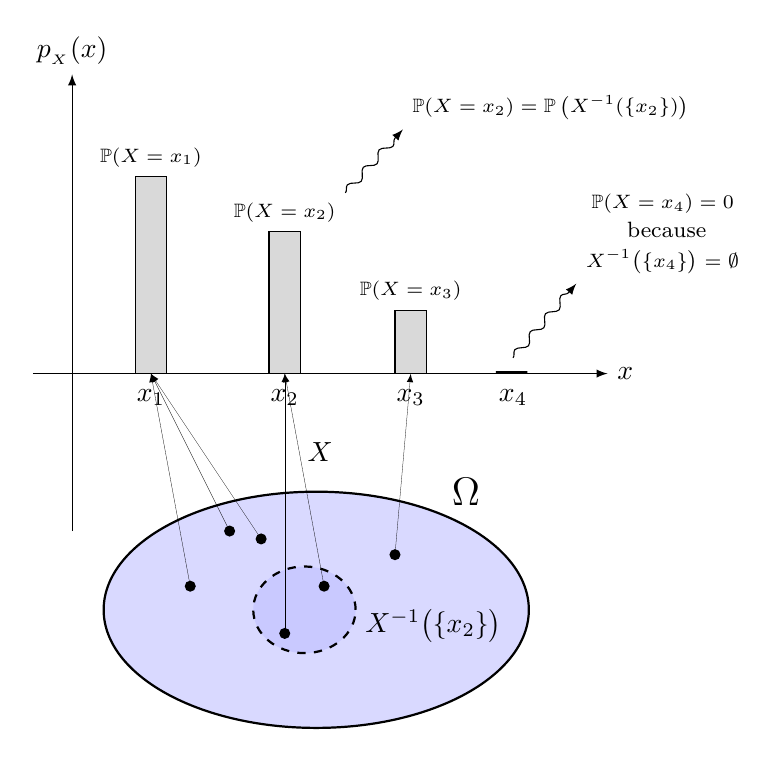
\begin{tikzpicture}[>=latex, scale=1.0]

% Axes
\draw[->] (-0.5,0) -- (6.8,0) node[right] {$x$};
\draw[->] (0,-2) -- (0,3.8) node[above] {$p_{_X}(x)$};

% x-values
\node at (1,-0.3) {$x_1$};
\node at (2.7,-0.3) {$x_2$};
\node at (4.3,-0.3) {$x_3$};
\node at (5.6,-0.3) (pointx4) {$x_4$};

% Histogram bars
\draw[fill=gray!30] (0.8,0) rectangle (1.2,2.5);
\draw[fill=gray!30] (2.5,0) rectangle (2.9,1.8);
\draw[fill=gray!30] (4.1,0) rectangle (4.5,0.8);
\draw[fill=gray!30, thick] (5.38,0.02) rectangle (5.78,0.02); % thin zero-height bar

% PMF labels above bars
\node[above, font=\scriptsize] at (1,2.5) {$\mathbb{P}(X=x_1)$};
\node[above, font=\scriptsize] at (2.7,1.8) (px2) {$\mathbb{P}(X=x_2)$};
\node[above, font=\scriptsize] at (4.3,0.8) {$\mathbb{P}(X=x_3)$};

%  Probability explanation label
\node[above right, font=\scriptsize] (exp2) at (4.2,3.1) 
    {$\mathbb{P}(X=x_2)=\mathbb{P}\left(X^{-1}(\{x_2\})\right)$};

% Squiggly arrow from PMF label to explanation label
\draw[->, thin, decorate, decoration={snake, amplitude=0.5mm, segment length=3mm}] 
    (px2.north east) -- (exp2.south west);

% Zero-probability explanation 
\node[below, font=\scriptsize] at (7.5,2.4) {$\mathbb{P}(X=x_4)=0$};
\node[font=\footnotesize] at (7.55,1.83) {because};
\node[below, font=\scriptsize] at (7.5,1.7) (px4) {$X^{-1}\big(\{x_4\}\big)=\emptyset$};

% Squiggly arrow from PMF to explanation label
\draw[->, thin, decorate, decoration={snake, amplitude=0.5mm, segment length=3mm}] 
    (5.6,0.2) -- (px4.south west);

% Omega set (draw FIRST)
\draw[thick, fill=blue!15] (3.1,-3.0) ellipse (2.7 and 1.5);
\node at (5,-1.5) {\Large $\Omega$};

% Subset X^{-1}(x2) (draw SECOND)
\draw[thick, dashed, fill=blue!30, fill opacity=0.4]
      (2.95,-3.0) ellipse (0.65 and 0.55);
\node[right] at (3.6,-3.2) {$X^{-1}\big(\{x_2\}\big)$};

% Sample points (draw LAST)
\fill (1.5,-2.7) circle (2pt);   % -> x1
\fill (2.4,-2.1) circle (2pt);   % -> x1
\fill (2,-2) circle (2pt);       % -> x1

\fill (2.7,-3.3) circle (2pt);   % -> x2
\fill (3.2,-2.7) circle (2pt);   % -> x2

\fill (4.1,-2.3) circle (2pt);   % -> x3

% Mapping arrows
\draw[->, ultra thin] (1.5,-2.7) -- (1,0);
\draw[->, ultra thin] (2.4,-2.1) -- (1,0);
\draw[->, ultra thin] (2,-2) -- (1,0);

\draw[->, ultra thin] (2.7,-3.3) -- (2.7,0);
\draw[->, ultra thin] (3.2,-2.7) -- (2.7,0);

\draw[->, ultra thin] (4.1,-2.3) -- (4.3,0);

% Label X
\node at (3.15,-1) {$X$};

		\end{tikzpicture}
\caption{Probability Law For a Discrete Random Variable.}
\label{fig:drvproblaw}	
	\end{center}
\end{figure}


\begin{defn}\label{def:continuous}
A random variable $X$ is called {\bf\emph{continuous}} if for every real number $x \in \mathbb{R}$,
\[
\mathbb{P}(X = x) = 0.
\]
Equivalently, the probability that $X$ lies in any interval $[a,b]$ is determined entirely by the cumulative distribution function $F_X$ via
\[
\mathbb{P}(a \le X \le b) = F_X(b) - F_X(a),
\]
and no single point has positive probability.
\end{defn}

We are only interested in the most common type of continuous random variable, called an absolutely continuous random variable.\\

\begin{defn}\label{def:absolute_continuous}
A random variable $X$ is called {\bf\emph{absolutely continuous}} if there exists a non-negative, integrable function $f_X:\mathbb{R} \to [0,\infty)$, called the \emph{probability density function (pdf)}, such that for every Borel set $A \subseteq \mathbb{R}$,
\[\mathbb{P}(X \in A) = \int_A f_X(x)\, dx.\]
Equivalently, the cumulative distribution function $F_X$ of $X$ can be written as
\[F_X(x) = \mathbb{P}(X \le x) = \int_{-\infty}^{x} f_X(t)\, dt \quad \text{for all } x \in \mathbb{R}.\]
\end{defn}

\ni Some of the most important random variables encountered in probability modeling and statistical theory, such as the uniform distribution or the normal distribution, are continuous random variables. \\


\begin{figure}[h!]
	\begin{center}
		\includegraphics[scale=0.7]{continuous_distribution_plot.jpeg}
\caption{Distribution Function for a Continuous Random Variable.}
\label{fig:drvdistribution}
	\end{center}
\end{figure}	


\vskip 1cm
\hrule
\vskip 1cm

%%%%%%%%%%%%%%%%%%%%%%%%%%%%%%%%%%%%%%%%%%%%%%%%%%%%%%%%%%%%%%%%%%%%%%%%%%%%%%%%%%%%%%%%%%%%%%%%%%%%%%
\section*{Foundational Examples: General Random Variables}
%%%%%%%%%%%%%%%%%%%%%%%%%%%%%%%%%%%%%%%%%%%%%%%%%%%%%%%%%%%%%%%%%%%%%%%%%%%%%%%%%%%%%%%%%%%%%%%%%%%%%%

\paragraph*{Problem 1: Simple discrete random variable:}
Let \(\Omega = \{1,2,3,4,5,6\}\) where for all $\omega\in\Omega$ we have \(\mathbb{P}(\{\omega\}) = \frac{1}{6}\). Define
\[
X(\omega) = 
\begin{cases} 
1 & \text{if $\omega$ is even} \\
0 & \text{if $\omega$ is odd}
\end{cases}
\]

\textbf{Questions:}
\begin{enumerate}
    \item Compute \(X^{-1}(\{0\})\) and \(X^{-1}(\{1\})\).
    \item Compute \(\mathbb{P}(X=0)\) and \(\mathbb{P}(X=1)\).
    \item Compute \(\mathbb{P}(X \in \{0,1\})\).
\end{enumerate}

\begin{hintbox}
List the even and odd numbers in \(\Omega\); then find which \(\omega\) map to 0 and 1.
\end{hintbox}

\ifnum\printsol=1
\begin{solutionbox}
\begin{enumerate}
    \item \(X^{-1}(\{0\}) = \{1,3,5\}\), \quad \(X^{-1}(\{1\}) = \{2,4,6\}\)
    \item \(\mathbb{P}(X=0) = 1/2\), \quad \(\mathbb{P}(X=1) = 1/2\)
    \item \(\mathbb{P}(X \in \{0,1\}) = 1\)
\end{enumerate}
\end{solutionbox}

\fi

\paragraph*{Problem 2: Inverse image with intervals:}
Let \(\Omega = [0,1]\) with Lebesgue measure and define
\[X(\omega) = \begin{cases} 
0 & 0\le\omega < 1/2 \\
1 & 1/2\le\omega\le 1
\end{cases}\]

\textbf{Questions:}
\begin{enumerate}
    \item Compute \(X^{-1}(\{0\})\) and \(X^{-1}(\{1\})\).
    \item Compute \(\mathbb{P}(X=0)\) and \(\mathbb{P}(X=1)\).
    \item Compute \(\mathbb{P}(X \in \{0,1\})\).
    \item Compute \(X^{-1}([0,0.5])\).
\end{enumerate}

\begin{hintbox}
Draw the interval \([0,1]\) and mark where \(X(\omega) = 0\) and \(X(\omega) = 1\). Use lengths of intervals for probabilities.
\end{hintbox}

\ifnum\printsol=1
\begin{solutionbox}
\begin{enumerate}
    \item \(X^{-1}(\{0\}) = (0,1/2)\), \quad \(X^{-1}(\{1\}) = (1/2,1)\)
    \item \(\mathbb{P}(X=0) = 1/2\), \quad \(\mathbb{P}(X=1) = 1/2\)
    \item \(\mathbb{P}(X \in \{0,1\}) = 1\)
    \item \(X^{-1}([0,0.5]) = (0,1/2)\)
\end{enumerate}
\end{solutionbox}

\fi

\paragraph*{Problem 3: Mapping to multiple values:}
Let \(\Omega = [0,1]\) and \(X(\omega) = \lfloor 3 \omega \rfloor\).

\textbf{Questions:}
\begin{enumerate}
    \item List the possible values of \(X\).
    \item For each value \(x\), compute \(X^{-1}(\{x\})\).
    \item Compute \(\mathbb{P}(X=0), \mathbb{P}(X=1), \mathbb{P}(X=2)\).
\end{enumerate}

\begin{hintbox}
Divide \([0,1]\) into three intervals of length \(1/3\). Each interval corresponds to a value of \(X\).
\end{hintbox}

\ifnum\printsol=1
\begin{solutionbox}
\begin{enumerate}
    \item Possible values: \(0,1,2\)
    \item \(X^{-1}(\{0\}) = [0,1/3)\), \quad \(X^{-1}(\{1\}) = [1/3,2/3)\), \quad \(X^{-1}(\{2\}) = [2/3,1)\)
    \item \(\mathbb{P}(X=0) = 1/3\), \(\mathbb{P}(X=1) = 1/3\), \(\mathbb{P}(X=2) = 1/3\)
\end{enumerate}
\end{solutionbox}

\fi

\paragraph*{Problem 4: Composition and inverse image:}
Let \(\Omega = \mathbb{R}\), \(X(\omega) = \omega^2\), and \(A = [1,4]\).

\textbf{Questions:}
\begin{enumerate}
    \item Compute \(X^{-1}(A)\).
    \item Draw a picture illustrating \(X^{-1}(A)\) on the real line.
    \item If \(\mathbb{P}\) is standard normal, compute \(\mathbb{P}(X \in A)\).
\end{enumerate}

\begin{hintbox}
For \(X(\omega) \in [1,4]\), solve \(\omega^2 \in [1,4]\). Consider both positive and negative roots.
\end{hintbox}

\ifnum\printsol=1
\begin{solutionbox}
\begin{enumerate}
    \item \(X^{-1}(A) = [-2,-1] \cup [1,2]\)
    \item Picture: Two intervals symmetric about zero: \([-2,-1]\) and \([1,2]\)
    \item \(\mathbb{P}(X \in A) = \mathbb{P}(-2 \le Z \le -1) + \mathbb{P}(1 \le Z \le 2) = 2(\Phi(2)-\Phi(1))\)
\end{enumerate}
\end{solutionbox}

\fi

\paragraph*{Problem 5: General property of inverse image:}
Prove that for any random variable \(X\) and any set \(A \subseteq \mathbb{R}\):
\[X^{-1}(A^c) = (X^{-1}(A))^c, \quad X^{-1}\Big(\bigcup_i A_i\Big) = \bigcup_i X^{-1}(A_i)\]

\textbf{Questions:}
\begin{enumerate}
    \item Prove the complement property.
    \item Prove the union property.
\end{enumerate}

\begin{hintbox}
Use the definition \(X^{-1}(A) = \{\omega : X(\omega) \in A\}\) and basic set operations.
\end{hintbox}

\ifnum\printsol=1
\begin{solutionbox}
\begin{itemize}
    \item \(X^{-1}(A^c) = \{\omega : X(\omega) \in A^c\} = \{\omega : X(\omega) \notin A\} = (X^{-1}(A))^c\)
    \item \(X^{-1}(\bigcup_i A_i) = \{\omega : X(\omega) \in \bigcup_i A_i\} = \bigcup_i X^{-1}(A_i)\)
\end{itemize}
\end{solutionbox}

\fi

\paragraph*{Problem 6: Random variable and probability inequalities:}
Let \(X\) be uniform on \([0,1]\), and define
\[Y = 1_{[0,1/3]}(X) = \begin{cases} 
1 & X \in [0,1/3] \\
0 & X \in (1/3,1]
\end{cases}\]

\textbf{Questions:}
\begin{enumerate}
    \item Compute \(Y^{-1}(\{1\})\) and \(Y^{-1}(\{0\})\).
    \item Compute \(\mathbb{P}(Y=1)\) and \(\mathbb{P}(Y=0)\).
    \item Verify \(\mathbb{P}(Y \in \{0,1\}) = 1\).
\end{enumerate}

\begin{hintbox}
Identify where \(Y = 1\) and where \(Y = 0\) on \([0,1]\). Then use interval lengths to compute probabilities.
\end{hintbox}

\ifnum\printsol=1
\begin{solutionbox}
\begin{enumerate}
    \item \(Y^{-1}(\{1\}) = [0,1/3]\), \quad \(Y^{-1}(\{0\}) = (1/3,1]\)
    \item \(\mathbb{P}(Y=1) = 1/3\), \(\mathbb{P}(Y=0) = 2/3\)
    \item \(\mathbb{P}(Y \in \{0,1\}) = 1\)
\end{enumerate}
\end{solutionbox}

\fi


\vskip 1cm
\hrule
\vskip 1cm


%%%%%%%%%%%%%%%%%%%%%%%%%%%%%%%%%%%%%%%%%%%%%%%%%%%%%%%%%%%%%%%%%%%%%%%%%%%%%%%%%%%%%%%%%%%%%%%%%%%%%%
\section*{Reflection: Why Inverse Images Matter}
%%%%%%%%%%%%%%%%%%%%%%%%%%%%%%%%%%%%%%%%%%%%%%%%%%%%%%%%%%%%%%%%%%%%%%%%%%%%%%%%%%%%%%%%%%%%%%%%%%%%%%

In the previous examples, probabilities involving the random variable $X$
were always computed using inverse images.

\medskip

\emph{Reflection Prompt:} In your own words, respond to the following:

\begin{itemize}
\item Why do we compute probabilities using $X^{-1}(A)$ rather than $X(A)$?
\item Where does probability \emph{actually live}: on the values of $X$ or on the sample space $\Omega$?
\item Describe one mistake a student might make if they confuse $X^{-1}(A)$ with $X(A)$.
\end{itemize}

\medskip

\ni Your response should focus on ideas and explanations rather than calculations.



\vskip 1cm
\hrule
\vskip 1cm

%%%%%%%%%%%%%%%%%%%%%%%%%%%%%%%%%%%%%%%%%%%%%%%%%%%%%%%%%%%%%%%%%%%%%%%%%%%%%%%%%%%%%%%%%%%%%%%%%%%%%%
\section*{Conceptual Quiz: Preimages of Random Variables}
%%%%%%%%%%%%%%%%%%%%%%%%%%%%%%%%%%%%%%%%%%%%%%%%%%%%%%%%%%%%%%%%%%%%%%%%%%%%%%%%%%%%%%%%%%%%%%%%%%%%%%

The purpose of this quiz is to reinforce the idea that probabilities involving a random variable
are computed using inverse images:
\[
\mathbb P(X\in A)=\mathbb P\big(X^{-1}(A)\big).
\]

\medskip

\textbf{Question:} Let $\Omega=(0,1)$ with the uniform probability measure.
Define a random variable $X:\Omega\to\mathbb R$ by
\[
X(\omega)=
\begin{cases}
-1, & 0<\omega<0.2,\\[4pt]
0,  & 0.2\le \omega<0.7,\\[4pt]
1,  & 0.7\le \omega<1.
\end{cases}
\]

Let $A=\{-1,1\}$.

\medskip

\begin{enumerate}
\item[(a)] Which of the following sets is \emph{exactly} $X^{-1}(A)$?

\[
\begin{array}{ll}
\text{(i)} & (0,0.2)\cup(0.7,1) \\[4pt]
\text{(ii)} & \{-1,1\} \\[4pt]
\text{(iii)} & (0,1)\setminus[0.2,0.7) \\[4pt]
\text{(iv)} & (0.2,0.7)
\end{array}
\]

\item[(b)] In one or two sentences, explain \emph{why} your choice in part (a) is correct.

\item[(c)] Without performing any calculations, explain how you would compute
\[
\mathbb P(X\in A).
\]

\item[(d)] What is the set $X(A)$? Is this set useful for computing probabilities?
Briefly explain.
\end{enumerate}

\medskip

\begin{solutionbox}
\begin{enumerate}
\item[(a)] The correct answer is \textbf{(i)}:
\[
X^{-1}(\{-1,1\})=(0,0.2)\cup(0.7,1).
\]

\item[(b)] The inverse image consists of all outcomes $\omega\in\Omega$ whose
assigned value under $X$ lies in the set $\{-1,1\}$.

\item[(c)] We compute
\[
\mathbb P(X\in A)=\mathbb P\big(X^{-1}(A)\big)
\]
by finding the probability (length) of the subset
$(0,0.2)\cup(0.7,1)\subset(0,1)$.

\item[(d)] The image of the set $A$ is
\[
X(A)=\{X(-1),X(1)\}.
\]
However, $-1$ and $1$ are not elements of the sample space $\Omega=(0,1)$,
so $X(A)$ is not meaningful in this context.

Even when $A\subset\Omega$, the set $X(A)$ lives in $\mathbb R$ and does not correspond
to an event in the sample space. Probabilities are always assigned to subsets of $\Omega$,
which is why inverse images are essential.
\end{enumerate}
\end{solutionbox}

\vskip 1cm
\hrule
\vskip 1cm

%%%%%%%%%%%%%%%%%%%%%%%%%%%%%%%%%%%%%%%%%%%%%%%%%%%%%%%%%%%%%%%%%%%%%%%%%%%%%%%%%%%%%%%%%%%%%%%%%%%%%%
\section*{Proofs of Theorems:}
%%%%%%%%%%%%%%%%%%%%%%%%%%%%%%%%%%%%%%%%%%%%%%%%%%%%%%%%%%%%%%%%%%%%%%%%%%%%%%%%%%%%%%%%%%%%%%%%%%%%%%

\begin{thm*}
Let $(\O,\F,\P)$ be a probability space and $X:\F\to\
R$ be a random variable with distribution function $F_{_X}$. Then the following properties hold.

	\begin{enumerate}
	
		\item $\ds\lim_{x\to-\infty}F_{_X}(x)=0$;
		\item $\ds\lim_{x\to\infty}F_{_X}(x)=1$;
		\item $F_{X}$ is monotonically increasing everywhere; i.e., if $x\le y$, then $F_{_X}(x)\le F_{_X}(y)$.
		\item $F_{X}$ is right-continuous; i.e., for all $x\in\R$ we have 
$\ds\lim_{\epsilon\to 0^+}F_{_X}(x+\epsilon)=F_{_X}(x)$. 
		
	\end{enumerate}
	
\end{thm*}

 
\begin{proof}
For property(1) we have
\[\ds\lim_{x\to-\infty}F_{_X}(x)=\ds\lim_{x\to-\infty}\P\Big(\left\{\o\in\O:X(\o)\le x\right\}\Big).\]
Now let $\{x_n\}$ be a sequence of real numbers such that $x_n\to-\infty$ as $n\to\infty$. Then let $A_n$ be the event $\{\o\in\O:X(\o)\le x_n\}$ so that $\{A_n\}$ is a decreasing sequence of events. Then we have 
\beq
\ds\lim_{x\to-\infty}F_{_X}(x)&=&\ds\lim_{x\to-\infty}\P\Big(\left\{\o\in\O:X(\o)\le x\right\}\Big)\\
&=&\ds\lim_{n\to\infty}\P\Big(\left\{\o\in\O:X(\o)\le x_n\right\}\Big)\\
&=&\ds\lim_{n\to\infty}\P\Big(A_n\Big)\\
&=&\P\left(\ds\bigcap^{\infty}_{n=1}A_n\right)\\
&=&\P\Big(\emptyset\Big)\\
&=&0
\eeq
This completes the proof of property(1). The proof of property(2) is very similar to that of property(1) and so we omit if for these notes. The proof of property(3) is trivial since if $x\le y$ we have $\{\o\in\O:X(\o)\le x\}\subseteq\{\o\in\O:X(\o)\le y\}$ and the result follows from monotonicity of probability measures. To show property(4) we let $\{\epsilon_n\}$ be any sequence so that $\epsilon_n\to 0$ as $n\to\infty$, and for a fixed $x\in\R$, let $A_n$ be the event $\{\o\in\O:X(\o)\le x+\epsilon_n\}$. Then consider
\beq
\ds\lim_{n\to\infty}F_{_X}(x+\epsilon_n)&=&\ds\lim_{n\to\infty}\P\Big(X\le x+\epsilon_n\Big)\\
&=&\ds\lim_{n\to\infty}\P\Big(A_n\Big)\\
&=&\P\left(\ds\bigcap^{\infty}_{n=1}A_n\right)\\
&=&\P\Big(\big\{\o\in\O:X(\o)\le x\big\}\Big)\\
&=&F_{_X}(x)\\
\eeq

\end{proof}

\ni{\bf\emph{Note}}: Some distribution functions, such as for a continuous random variable, will be left-continuous; i.e., and so continuous, but many random variables, such as discrete random variables will not be left-continuous.\\



%%%%%%%%%%%%%%%%%%%%%%%%%%%%%%%%%%%%%%%%%%%%%%%%%%%%%%%%%%%%%%%%%%%%%%%%%%%%%%%%%%%%%%%%%%%%%%%%%%%%%%%
%\section*{The R Code:} 
%%%%%%%%%%%%%%%%%%%%%%%%%%%%%%%%%%%%%%%%%%%%%%%%%%%%%%%%%%%%%%%%%%%%%%%%%%%%%%%%%%%%%%%%%%%%%%%%%%%%%%%
% Here is the R code used for the above simulations.
%\vspace*{2mm}
%\small 
%\begin{lstlisting}[language=R]
%
%
%
%\end{lstlisting}



\vskip 1cm
\hrule
\vskip 5mm
\begin{center}
\bf Please let me know if you have any questions, comments, or corrections!
\end{center}

%%%%%%%%%%%%%%%%%%%%%%%%%%%%%%%%%%%%%%%%%%%%%%%%%%%%%%
\end{document}
%%%%%%%%%%%%%%%%%%%%%%%%%%%%%%%%%%%%%%%%%%%%%%%%%%%%%%
